\clearpage
\section{Study of exploration intrinsic rewards} 
\label{sec:study_intrinsic_reward}
\begin{figure}[h]
    \centering
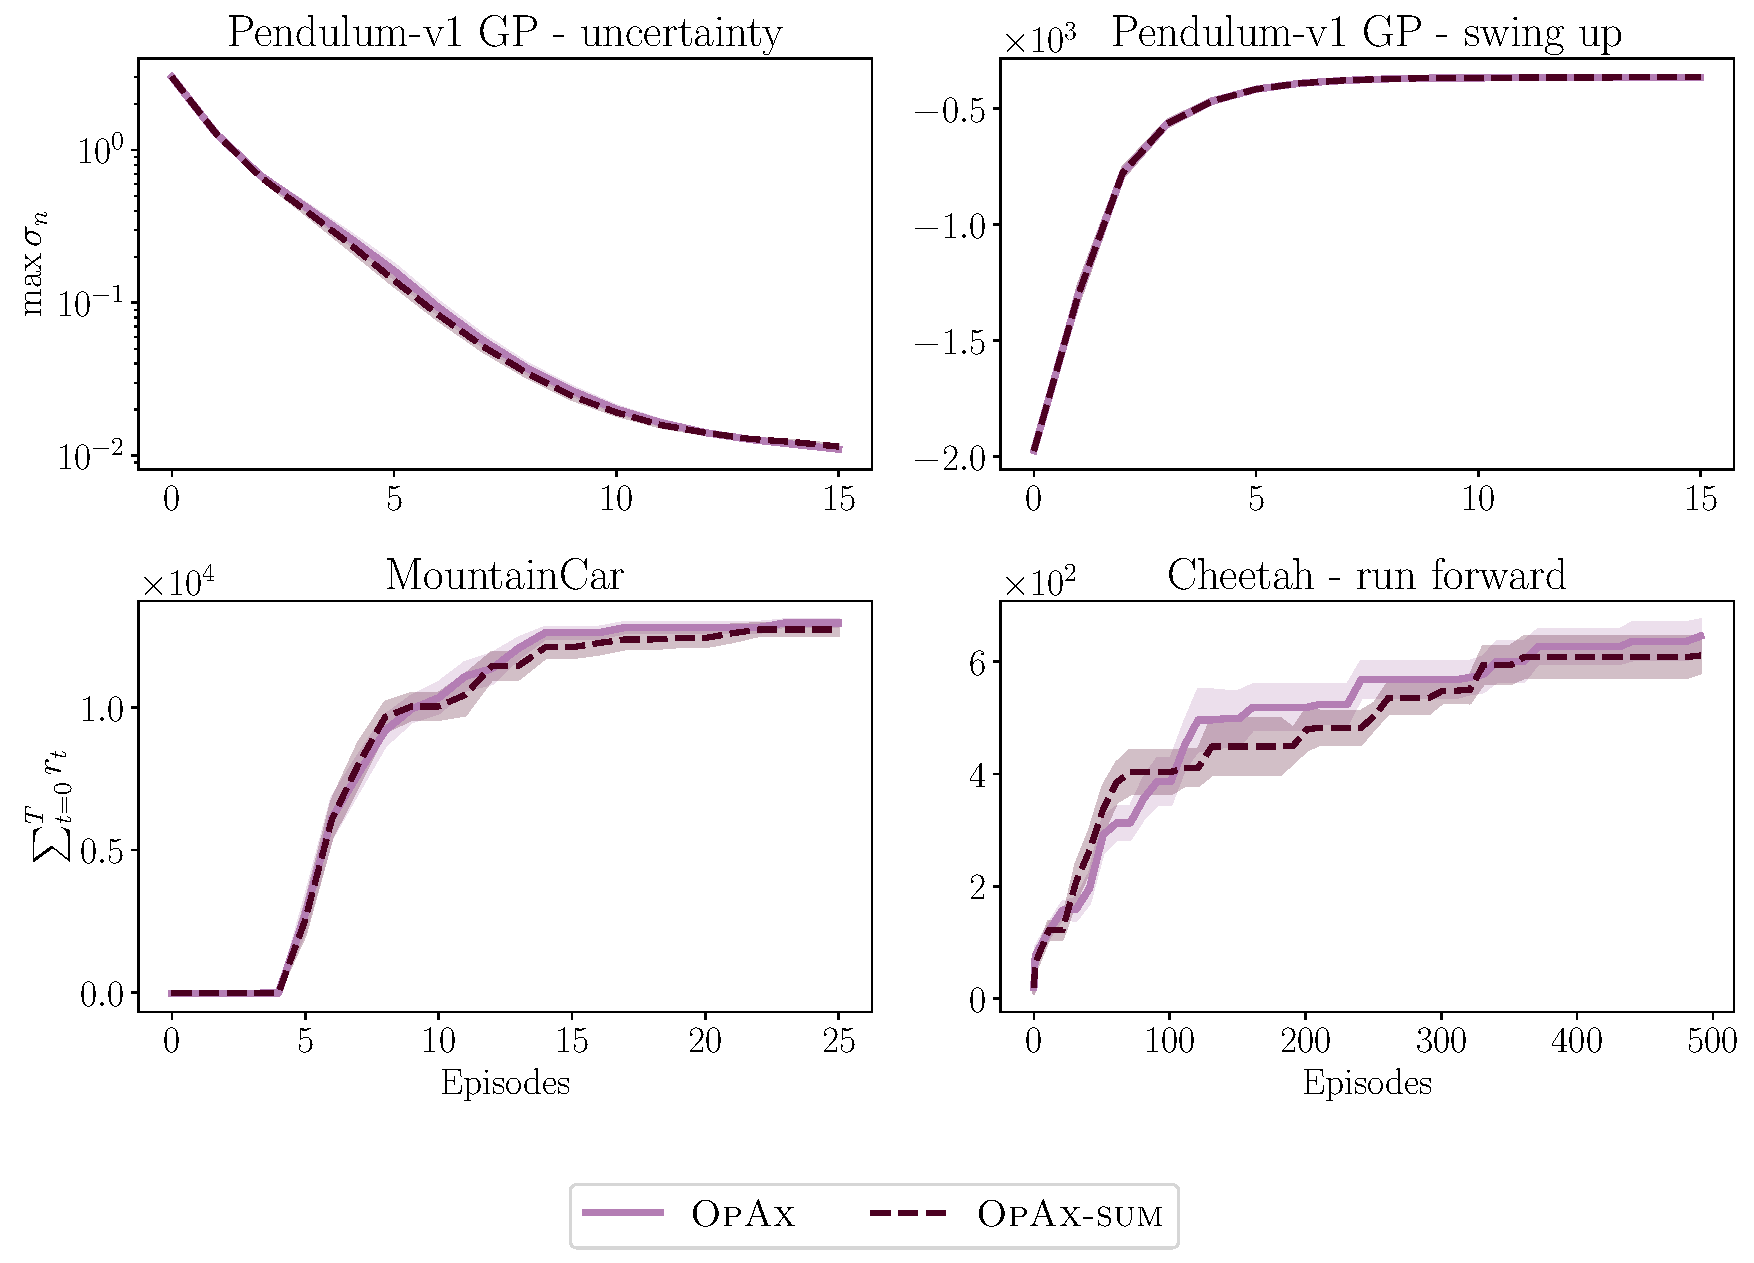
\includegraphics[width=0.8\textwidth]{figures/sum_rewards_comparison.pdf}
    \caption{Comparison of \opacex between intrinsic reward proposed in \Cref{eq:exploration_op} and the sum of epistemic uncertainties proposed by~\citep{pathak2019self}, i.e., \opacex-\textsc{sum}. For both choices of intrinsic rewards, \opacex reduces the epistemic uncertainty and performs well on downstream tasks.}
    \label{fig:comparison_sum}
\end{figure}
The intrinsic reward suggested in \Cref{eq:exploration_op} takes the log of the model epistemic uncertainty. Another common choice for the intrinsic reward is the epistemic uncertainty or model disagreement without the log~\citep{pathak2019self, sekar2020planning}. In the following Lemma, we show that these rewards are closely related.
\begin{lemma}
    Let  $\sigma_{\max} = \sup_{\vz \in \setZ; i \geq 0; 1\leq j\leq d_x} \sigma_{i, j}(\vz)$ and $\sigma >  0$. Then for all $i\geq 0$ and $j \in \{1, \dots, d_x\}$
    \begin{equation*}
        \sigma^2_{i, j}(\vz) \leq \frac{\sigma_{\max}}{\log(1 + \sigma^{-2}\sigma_{\max})}\log(1 + \sigma^{-2}\sigma^2_{i, j}(\vz)) \leq \frac{\sigma^{-2}\sigma_{\max}}{\log(1 + \sigma^{-2}\sigma_{\max})} \sigma^2_{i, j}(\vz). 
    \end{equation*}
\end{lemma}
\begin{proof}
\cite{curi2020efficient}  derive the first inequality on the left. The second inequality follows since $\log(1 + x) \leq x$ for all $x \geq 0$.
\end{proof}
\looseness=-1
Due to this close relation between the two objectives, our theoretical findings also apply to the intrinsic reward proposed by~\citep{pathak2019self}. Moreover, empirically we notice in~\Cref{fig:comparison_sum} that \opacex performs similarly when the sum of epistemic uncertainties is used instead of the objective in \Cref{eq:exploration_op}. However, our objective can naturally be extended to the case of heteroscedastic aleatoric noise, since it trades off the ratio of epistemic and aleatoric uncertainty.